\section{Network Design and Architecture}
\begin{figure}[h]
	\centering
	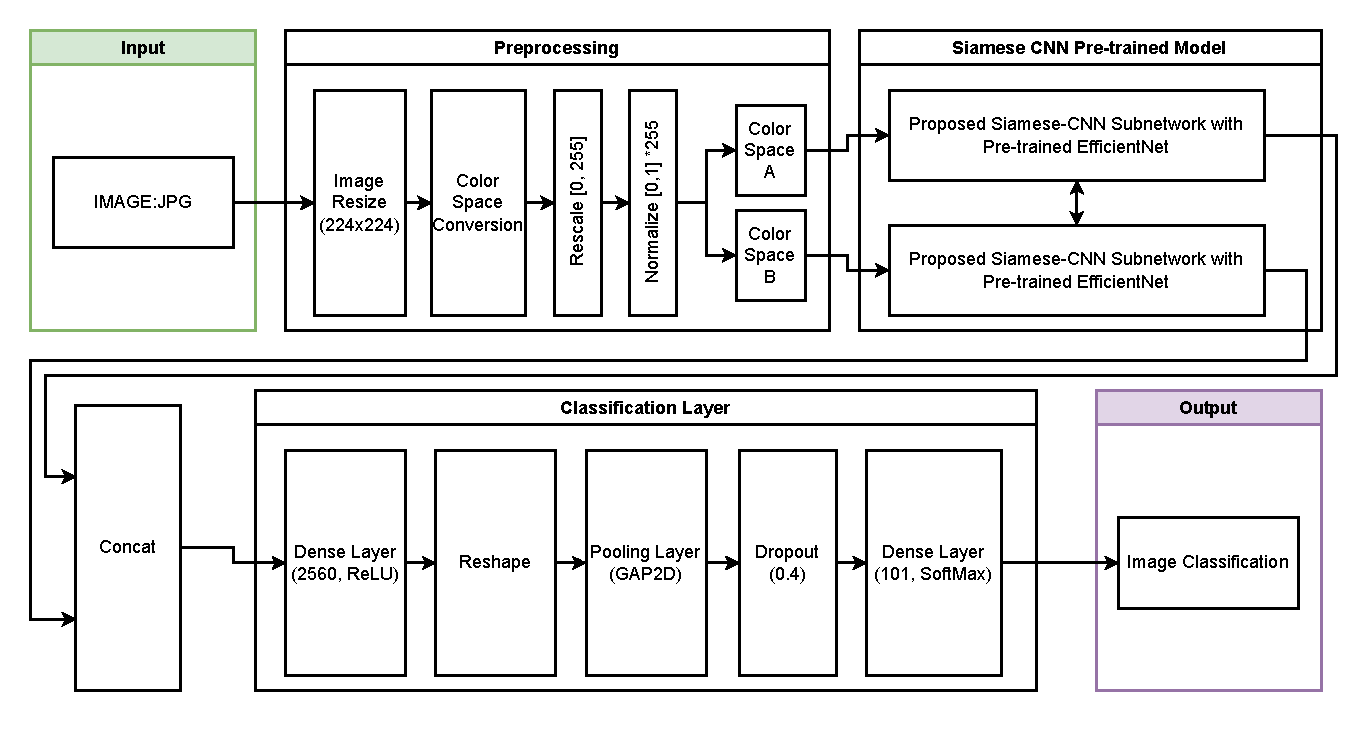
\includegraphics[width=1.0\textwidth]{graphics/images/Proposed_Model.pdf}
	\caption{FoodWhizNet Framework}
	\label{fig:proposedmodel}
\end{figure}

The proposed model will utilize the EfficientNet model family to be fine-tuned to specifically adapt the food image classification problem. This particular model family focuses on balancing the network resolution, width, and depth to achieve a better performance compared to the other ConvNets while considering resources \cite{ pmlr-v97-tan19a}. The study will be utilizing EfficientNet as the base model, starting with EfficientNetB0, the baseline of the EfficientNet family. The structure of EfficientNetB0 is shown in the Figure \ref{fig:efficientNetB0}. The base model will initially use the weights from the ImageNet database, which is a large-scale image database with up to 14 million images. The base model will mainly be used as the primary model in each subnetwork of the proposed Siamese CNN model. The top layer of the base model is removed, which is the fully connected layer, and beyond that, shown inside a red box in Figure \ref{fig:efficientNetB0}. This is to give a problem-specific classification layer, in this case, the image classification problem. The study will also go through all the EfficientNet family to test each of the series as the base model for the proposed model.

\begin{figure}[h]
	\centering
	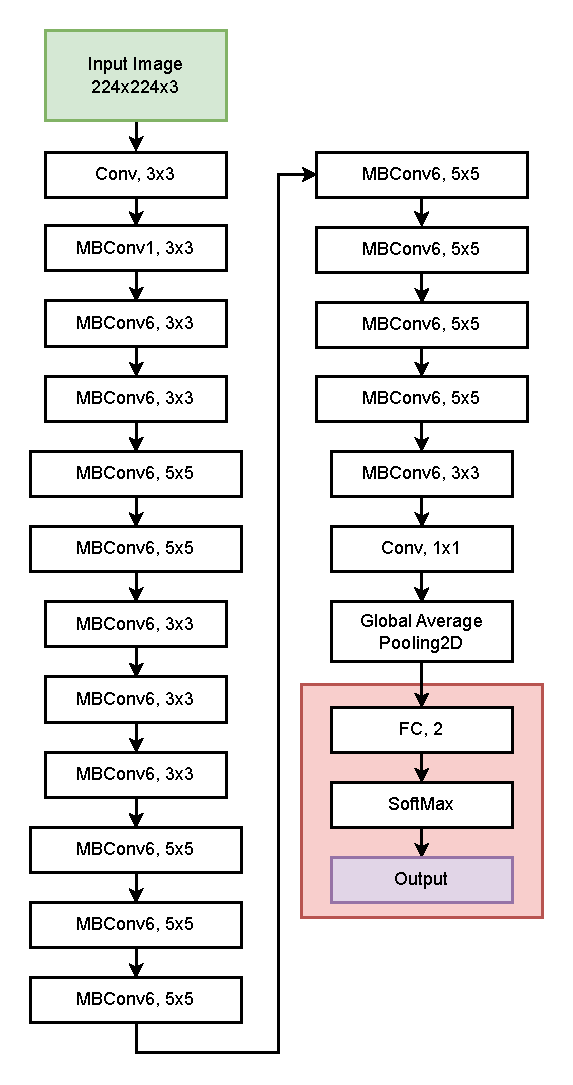
\includegraphics[width=0.5\textwidth]{graphics/images/EfficientNetB0.pdf}
	\caption{EfficientNetB0 Architecture with top layer in red box}
	\label{fig:efficientNetB0}
\end{figure}

Before utilizing the base model, three data augmentation layers are added. These are random rotation, random translation, and random flipping. These data augmentation layers are only activated during the training phase of the model and never during the testing phase. In addition to fine-tuning the pre-trained base model, a Global Average Pooling 2D layer is added, and a Dropout layer with a dropout rate of 0.3 is also added afterward. This completes the fine-tuning of the base model which is to be used in the base subnetwork of the proposed Siamese CNN model. Figure \ref{fig:pscnnsn} shows a diagram of the base subnetwork of the proposed Siamese CNN.

\begin{figure}[h]
	\centering
	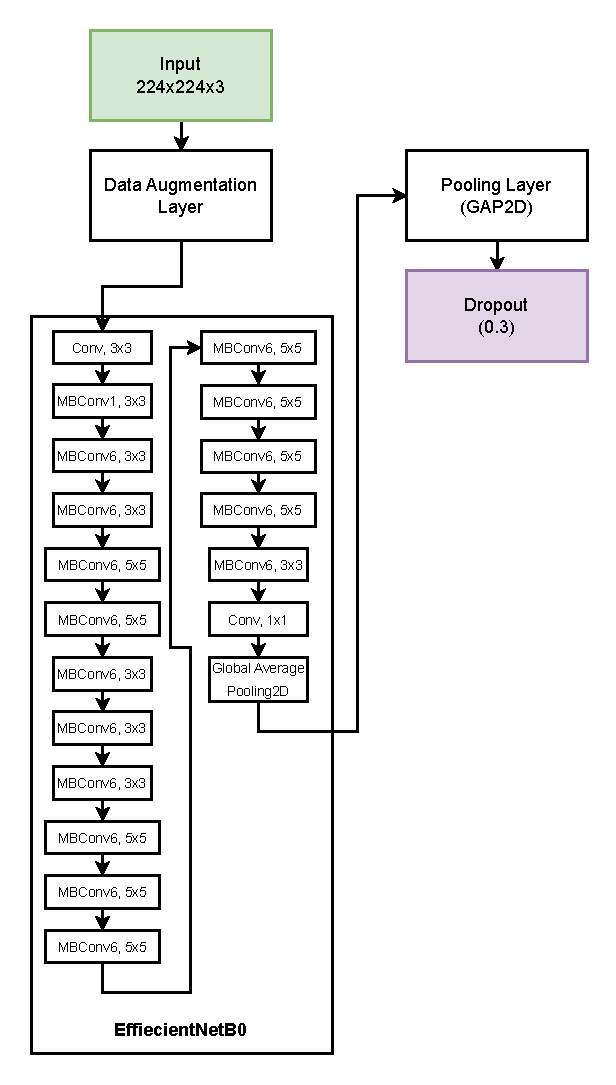
\includegraphics[width=0.5\textwidth]{graphics/images/Proposed-SCNN-Subnetwork.pdf}
	\caption{Proposed Siamese-CNN Subnetwork with pre-trained EfficientNetB0}
	\label{fig:pscnnsn}
\end{figure}

To complete the whole Siamese CNN model, two of the base subnetworks are created and then a Concat layer is instantiated with the subnetworks as inputs. Another fine-tuning is conducted after the Concat layer with an additional Dense layer of 2560 units and ReLU activation, a Global Average Pooling 2D layer, a Dropout layer with a rate of 0.4, and finally a Dense layer for the final fully connected layer with 101 units and with a SoftMax activation function. Figure \ref{fig:proposedmodel} shows an overview of the proposed Siamese CNN model. The model accepts two inputs each will be fed on each subnetwork.

\section{Dataset}
The dataset to be used in this study is the Food-101\cite{bossard-2014}. It was first used to conduct a study with regards to mining discriminative features using a novel approach called the Random Forest for machine learning \cite{bossard-2014}. Since the dataset has its ground truth, no validation set was presented when using it. Therefore, it has no predefined split like the training, validation, and evaluation. It was set as a whole, giving the user much more control in terms of utilizing it for a split. The dataset is structured into 101 classes of various foods containing a thousand image samples in JPG format in each class, producing 101000 samples in total. Each image is labeled and identified accordingly. A sample instance from the dataset is shown in \ref{fig:sampleimg}. This particular instance is labeled \textit{huevos\_rancheros/614968}. The first part of its label is the class name it is part of and the second part is its instance ID.

\begin{figure}[h]
	\centering
	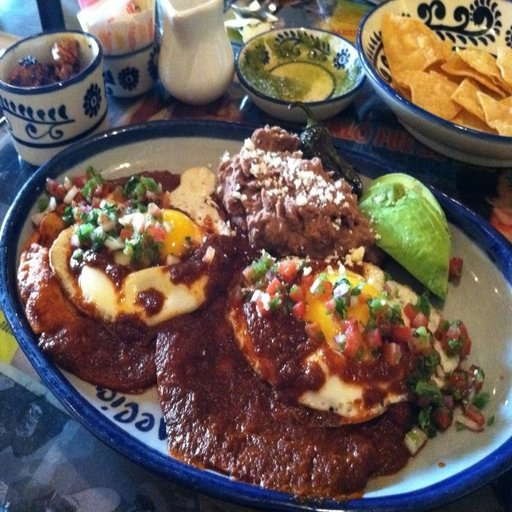
\includegraphics[width=0.5\textwidth]{graphics/images/sample_image.jpg}
	\caption{A sample instance labeled huevos\_rancheros/614968}
	\label{fig:sampleimg}
\end{figure}

The splitting of the dataset will follow the related studies \cite{pandey-2017,vijayakumari-2022,martinel-2018}. The common and most recommended way to split the dataset is by allocating samples for training, validation, and evaluation, but the studies that utilized the Food101 dataset only include the training and evaluation sets which are conducted using the 75-25 split. Since the total number of samples in the dataset is 101000, 75750 of them are allocated for the training phase and 25250 samples are to be utilized in the evaluation phase. Shown in Figure \ref{fig:dss} is the process of splitting the dataset. 

\begin{figure}[h]
	\centering
	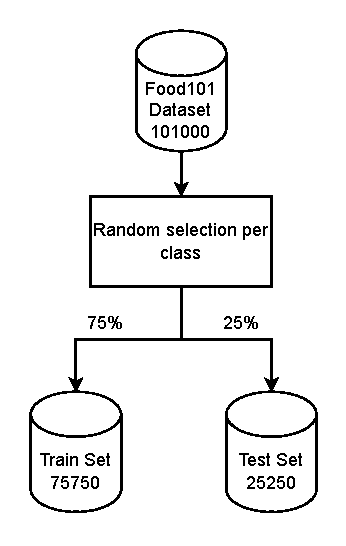
\includegraphics[width=0.5\textwidth]{graphics/images/DatasetSplit.pdf}
	\caption{Dataset Split}
	\label{fig:dss}
\end{figure}

Table \ref{tab:dataprofile} shows the data profile of the primary dataset. In the first column are the names of the classes which are the 101 food names. The second column indicates the total instances in each class which is uniform across all classes to be 1000 instances. The third column includes the number of instances in each class that will be used for the training of the model. In this case, since 75\% of each class is for training, therefore 750 instances per class are selected. The fourth column is the 25\%  remaining instances bound for the evaluation phase. The split is predetermined by the existing literature \cite{bossard-2014}. 

\begin{center}
    \begin{longtable}{|l|l|l|l|}
        \captionsetup{singlelinecheck=false, justification=raggedright, labelfont=bf}
        \caption{Food-101 Dataset Profile.} \label{tab:dataprofile} \\
        \hline
        \textbf{Class Name} & \textbf{Total Instances} & \textbf{Training Instances} & \textbf{Testing Instances} \\
        \hline
        \endfirsthead
    
        \multicolumn{4}{l}% 
        {{\bfseries \tablename\ \thetable{} -- continued from previous page}} \\ 
        \hline
        \textbf{Class Name} & \textbf{Total Instances} & \textbf{Training Instances} & \textbf{Testing Instances} \\
        \hline
        \endhead
    
        \hline \multicolumn{4}{|r|}{{Continued on next page}} \\ 
        \hline
        \endfoot
    
        \hline 
        \hline
        \endlastfoot
    
        apple pie & 1000 & 750 & 250 \\
        baby back ribs & 1000 & 750 & 250 \\
        baklava & 1000 & 750 & 250 \\
        beef carpaccio & 1000 & 750 & 250 \\
        beef tartare & 1000 & 750 & 250 \\
        beet salad & 1000 & 750 & 250 \\
        beignets & 1000 & 750 & 250 \\
        bibimbap & 1000 & 750 & 250 \\
        bread pudding & 1000 & 750 & 250 \\
        breakfast burrito & 1000 & 750 & 250 \\
        bruschetta & 1000 & 750 & 250 \\
        caesar salad & 1000 & 750 & 250 \\
        cannoli & 1000 & 750 & 250 \\
        caprese salad & 1000 & 750 & 250 \\
        carrot cake & 1000 & 750 & 250 \\
        ceviche & 1000 & 750 & 250 \\
        cheesecake & 1000 & 750 & 250 \\
        cheese plate & 1000 & 750 & 250 \\
        chicken curry & 1000 & 750 & 250 \\
        chicken quesadilla & 1000 & 750 & 250 \\
        chicken wings & 1000 & 750 & 250 \\
        chocolate cake & 1000 & 750 & 250 \\
        chocolate mousse & 1000 & 750 & 250 \\
        churros & 1000 & 750 & 250 \\
        clam chowder & 1000 & 750 & 250 \\
        club sandwich & 1000 & 750 & 250 \\
        crab cakes & 1000 & 750 & 250 \\
        creme brulee & 1000 & 750 & 250 \\
        croque madame & 1000 & 750 & 250 \\
        cup cakes & 1000 & 750 & 250 \\
        deviled eggs & 1000 & 750 & 250 \\
        donuts & 1000 & 750 & 250 \\
        dumplings & 1000 & 750 & 250 \\
        edamame & 1000 & 750 & 250 \\
        eggs benedict & 1000 & 750 & 250 \\
        escargots & 1000 & 750 & 250 \\
        falafel & 1000 & 750 & 250 \\
        filet mignon & 1000 & 750 & 250 \\
        fish and chips & 1000 & 750 & 250 \\
        foie gras & 1000 & 750 & 250 \\
        french fries & 1000 & 750 & 250 \\
        french onion soup & 1000 & 750 & 250 \\
        french toast & 1000 & 750 & 250 \\
        fried calamari & 1000 & 750 & 250 \\
        fried rice & 1000 & 750 & 250 \\
        frozen yogurt & 1000 & 750 & 250 \\
        garlic bread & 1000 & 750 & 250 \\
        gnocchi & 1000 & 750 & 250 \\
        greek salad & 1000 & 750 & 250 \\
        grilled cheese sandwich & 1000 & 750 & 250 \\
        grilled salmon & 1000 & 750 & 250 \\
        guacamole & 1000 & 750 & 250 \\
        gyoza & 1000 & 750 & 250 \\
        hamburger & 1000 & 750 & 250 \\
        hot and sour soup & 1000 & 750 & 250 \\
        hot dog & 1000 & 750 & 250 \\
        huevos rancheros & 1000 & 750 & 250 \\
        hummus & 1000 & 750 & 250 \\
        ice cream & 1000 & 750 & 250 \\
        lasagna & 1000 & 750 & 250 \\
        lobster bisque & 1000 & 750 & 250 \\
        lobster roll sandwich & 1000 & 750 & 250 \\
        macaroni and cheese & 1000 & 750 & 250 \\
        macarons & 1000 & 750 & 250 \\
        miso soup & 1000 & 750 & 250 \\
        mussels & 1000 & 750 & 250 \\
        nachos & 1000 & 750 & 250 \\
        omelette & 1000 & 750 & 250 \\
        onion rings & 1000 & 750 & 250 \\
        oysters & 1000 & 750 & 250 \\
        pad thai & 1000 & 750 & 250 \\
        paella & 1000 & 750 & 250 \\
        pancakes & 1000 & 750 & 250 \\
        panna cotta & 1000 & 750 & 250 \\
        peking duck & 1000 & 750 & 250 \\
        pho & 1000 & 750 & 250 \\
        pizza & 1000 & 750 & 250 \\
        pork chop & 1000 & 750 & 250 \\
        poutine & 1000 & 750 & 250 \\
        prime rib & 1000 & 750 & 250 \\
        pulled pork sandwich & 1000 & 750 & 250 \\
        ramen & 1000 & 750 & 250 \\
        ravioli & 1000 & 750 & 250 \\
        red velvet cake & 1000 & 750 & 250 \\
        risotto & 1000 & 750 & 250 \\
        samosa & 1000 & 750 & 250 \\
        sashimi & 1000 & 750 & 250 \\
        scallops & 1000 & 750 & 250 \\
        seaweed salad & 1000 & 750 & 250 \\
        shrimp and grits & 1000 & 750 & 250 \\
        spaghetti bolognese & 1000 & 750 & 250 \\
        spaghetti carbonara & 1000 & 750 & 250 \\
        spring rolls & 1000 & 750 & 250 \\
        steak & 1000 & 750 & 250 \\
        strawberry shortcake & 1000 & 750 & 250 \\
        sushi & 1000 & 750 & 250 \\
        tacos & 1000 & 750 & 250 \\
        takoyaki & 1000 & 750 & 250 \\
        tiramisu & 1000 & 750 & 250 \\
        tuna tartare & 1000 & 750 & 250 \\
        waffles & 1000 & 750 & 250 \\
    \end{longtable}
\end{center}

\section{Data Processing}
In engaging with deep learning, the data must be preprocessed first for the model to utilize it efficiently. Preprocessing such as rescaling, reshaping, and other preprocessing methods are selected according to what suits best to the task that the study will be focusing on.

For this study, a particular preprocessing technique is conducted called the color space conversion. Since this study focuses on the multiple color space input to image classification, it is an important part to be considered.

Before conducting a color space conversion, the image must be resized first to the required dimension for the model to process. In the proposed model, the required size should be 224 x 224. After the resizing of each instance, a single instance will be subjected to two color space conversions of choice. Given the sample instance from figure \ref{fig:sampleimg}, it was converted to 11 color spaces as presented in figure \ref{fig:colorspaces}. 

\begin{figure}[htbp]
  \centering

  \begin{subfigure}[b]{0.22\textwidth}
    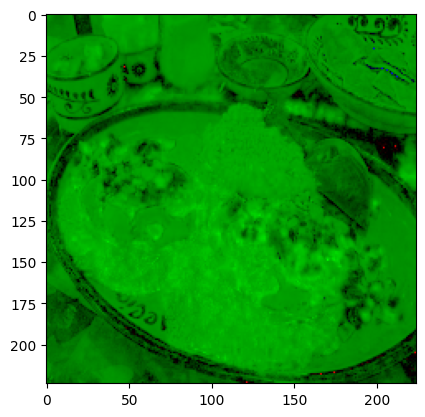
\includegraphics[width=\textwidth]{graphics/images/colorspaces/hed.png}
    \caption{HED}
    \label{fig:hed}
  \end{subfigure}
  \hfill
  \begin{subfigure}[b]{0.22\textwidth}
    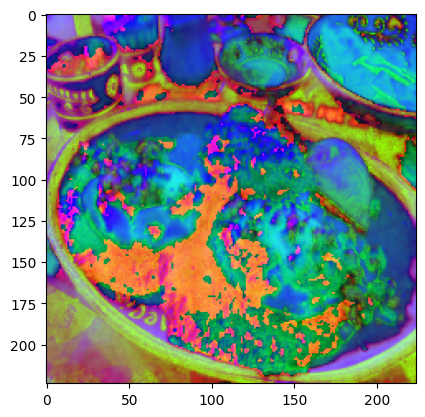
\includegraphics[width=\textwidth]{graphics/images/colorspaces/hsv.png}
    \caption{HSV}
    \label{fig:hsv}
  \end{subfigure}
  \hfill
  \begin{subfigure}[b]{0.22\textwidth}
    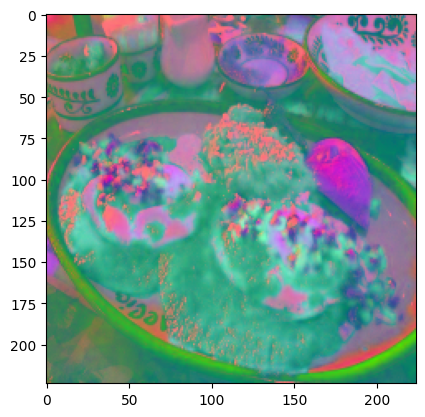
\includegraphics[width=\textwidth]{graphics/images/colorspaces/lab.png}
    \caption{LAB}
    \label{fig:lab}
  \end{subfigure}
  \hfill
  \begin{subfigure}[b]{0.22\textwidth}
    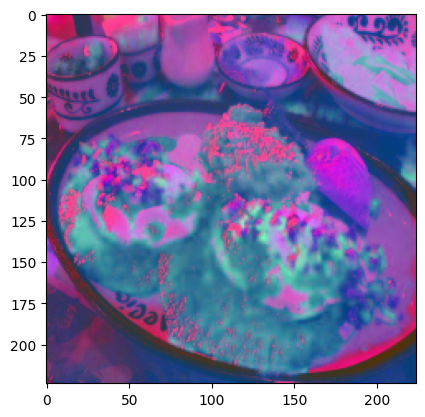
\includegraphics[width=\textwidth]{graphics/images/colorspaces/luv.png}
    \caption{LUV}
    \label{fig:luv}
  \end{subfigure}
  \hfill
  \medskip
  \begin{subfigure}[b]{0.22\textwidth}
    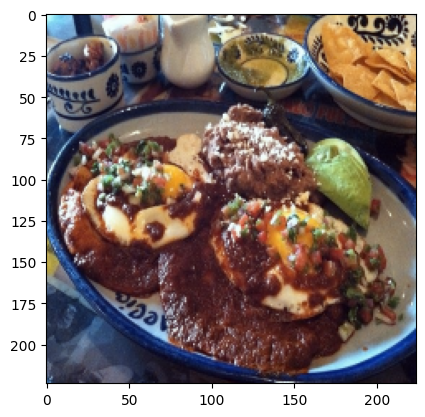
\includegraphics[width=\textwidth]{graphics/images/colorspaces/rgbcie.png}
    \caption{RGBCIE}
    \label{fig:rgbcie}
  \end{subfigure}
  \hfill
  \begin{subfigure}[b]{0.22\textwidth}
    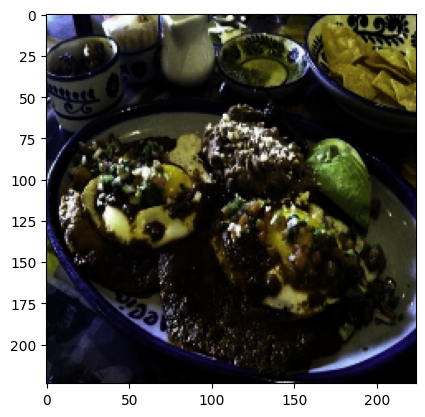
\includegraphics[width=\textwidth]{graphics/images/colorspaces/xyz.png}
    \caption{XYZ}
    \label{fig:xyz}
  \end{subfigure}
  \hfill
  \begin{subfigure}[b]{0.22\textwidth}
    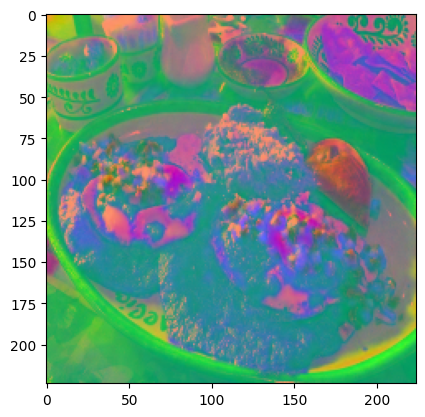
\includegraphics[width=\textwidth]{graphics/images/colorspaces/ycbcr.png}
    \caption{YCbCr}
    \label{fig:ycbcr}
  \end{subfigure}
  \hfill
  \begin{subfigure}[b]{0.22\textwidth}
    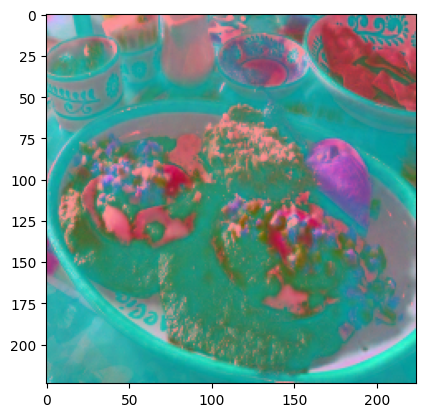
\includegraphics[width=\textwidth]{graphics/images/colorspaces/ydbdr.png}
    \caption{YDbDr}
    \label{fig:ydbdr}
  \end{subfigure}
  \hfill
  \medskip
  \begin{subfigure}[b]{0.22\textwidth}
    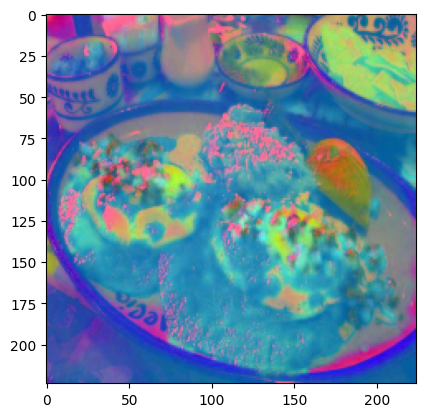
\includegraphics[width=\textwidth]{graphics/images/colorspaces/yiq.png}
    \caption{YIQ}
    \label{fig:yiq}
  \end{subfigure}
  \hfill
  \begin{subfigure}[b]{0.22\textwidth}
    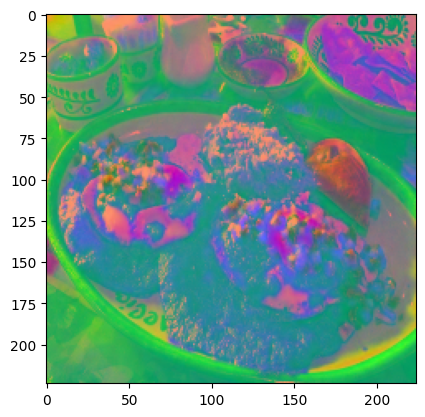
\includegraphics[width=\textwidth]{graphics/images/colorspaces/ypbpr.png}
    \caption{YPbPr}
    \label{fig:ypbpr}
  \end{subfigure}
  \hfill
  \begin{subfigure}[b]{0.22\textwidth}
    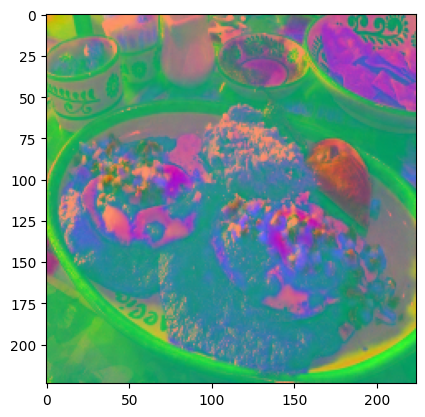
\includegraphics[width=\textwidth]{graphics/images/colorspaces/yuv.png}
    \caption{YUV}
    \label{fig:yuv}
  \end{subfigure}
 
  \caption{Images converted to color spaces}
  \label{fig:colorspaces}
\end{figure}

The conversion process also modifies the pixel values to sometimes include negative values. To address this, the function also normalizes the output image to a range [0, 255] which is necessary for the base model \cite{gangan-2022}. The image is first rescaled to the [0, 255] value range and then normalized to [0,1] to properly represent the converted image data. This will prevent the input data from being misrepresented. The normalized data is again converted to [0, 255] value range for the proposed model to process. Using the Min-Max Scaling as shown in Equation \ref{eq:mms} to normalize and rescale the image pixel data about the whole image. The output of the generic Min-Max Scaling is from [0,1] so a modification is done to achieve the [0,255] output range shown in Equation \ref{eq:mmsm}.

\begin{equation} \label{eq:mms}
X_{scaled} = \frac{X-X_{min}}{X_{max}-X_{min}}
\end{equation}
\begin{equation} \label{eq:mmsm}
X_{scaled} = \frac{X-X_{min}}{X_{max}-X_{min}} \cdot 255.0
\end{equation}

In the training phase of the model, the two converted images will be subjected to three data augmentation techniques. The random flipping, random rotation, and random translation are shown in figures \ref{fig:flipped}, \ref{fig:rotated}, and \ref{fig:translated}. Since they are in sequence, all three data augmentation techniques will result in figure \ref{fig:augmented}. Random flipping data augmentation technique is used to flip the image either horizontally, vertically, or both. Random Rotation is a data augmentation technique that rotates the image tensor to some degree. The Random Translation augmentation technique translates the image to some factor on its height and width. The use of data augmentation techniques ensures that the model sees a new instance of the sample and reduces overfitting. Some data augmentation layers are not utilized alone such as the RandomCrop layer since it produces a new shape which means an additional Reshape layer must be added to encourage more data augmentation techniques.

\begin{figure}[htbp]
  \centering

  \begin{subfigure}[b]{0.45\textwidth}
    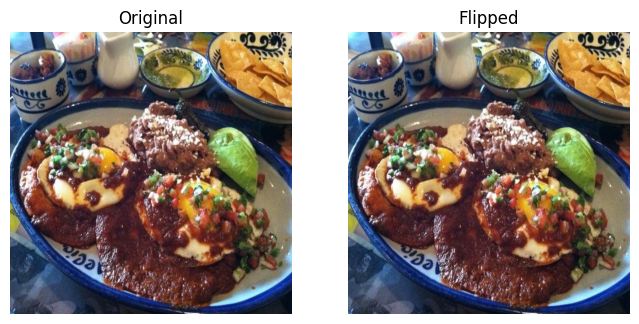
\includegraphics[width=\textwidth]{graphics/images/augmentation/flipped.png}
    \caption{Flip Augmentation}
    \label{fig:flipped}
  \end{subfigure}
  \hfill
  \begin{subfigure}[b]{0.45\textwidth}
    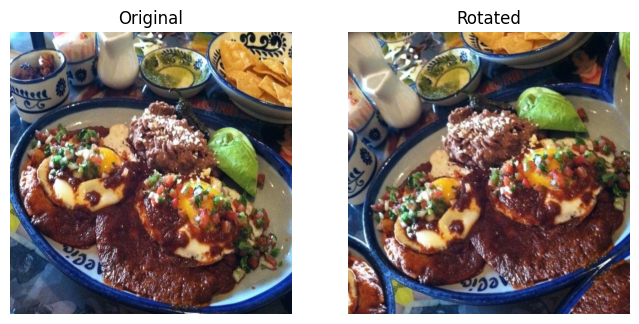
\includegraphics[width=\textwidth]{graphics/images/augmentation/rotated.png}
    \caption{Rotate Augmentation}
    \label{fig:rotated}
  \end{subfigure}
  \hfill
  \medskip
  \begin{subfigure}[b]{0.45\textwidth}
    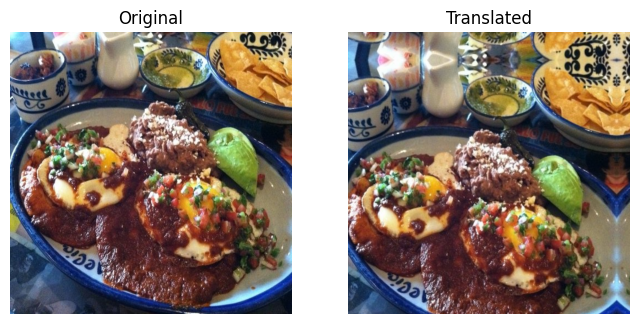
\includegraphics[width=\textwidth]{graphics/images/augmentation/translated.png}
    \caption{Translate Augmentation}
    \label{fig:translated}
  \end{subfigure}
  \hfill
  \begin{subfigure}[b]{0.45\textwidth}
    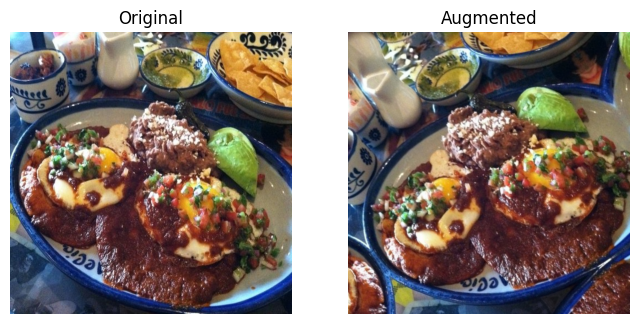
\includegraphics[width=\textwidth]{graphics/images/augmentation/augmented.png}
    \caption{The 3 augmentation}
    \label{fig:augmented}
  \end{subfigure}
  
  \caption{Images subjected to data augmentation}
  \label{fig:augmentation}
\end{figure}

\section{Model Training and Evaluation Details}
In training the model, the train split of the dataset is used. With 75\% of the total samples, the train set comprises of 75750 instances. Since each instances are converted to two color spaces, a total of 151500 instances are created but they come in pairs so there are still 75750 instances to be shuffled and batched. A batch size of 32 is used for this study and will be run on a 100-epoch limit to evaluate the baseline model. To know if the model is still learning and avoids wasting resources, 15\% of the test split is utilized per epoch to serve as a validation set.

A categorical loss function is used since this is a multiclass classification problem. This study will utilize the Categorical Cross-Entropy Loss function \cite{kumar-2018} which is defined in Equation \ref{eq:cce}. This is used to calculate the prediction disparity between the predicted value and the true value in the evaluation phase of the model. The\(p_i\) is the predicted probability of class i, which is the output of the softmax function. The \(y_i\) is the true value of the class. The summation of the true value dot product of the log of the predicted value is the standard cross-entropy formula as shown in the equation.

\begin{equation} \label{eq:cce}
CCE(p,y)= -\sum_{i=1}^{C} y_i\cdot log(p_i)
\end{equation}

An Adam optimizer is also used as an optimizer for training the model. Starting with a high learning rate of 0.01, decreasing by a factor of 0.2 when there is a plateau of validation accuracy until it reaches the lower learning rate limit of 1.0e-7. 

Callbacks are also utilized to assess the training. Specifically, the use of EarlyStopping callback to avoid wasting resources. This stops after no further improvement can be made to the validation accuracy of the training after 3 epochs. This also restores the best weight found across all runs. The ReduceLROnPlateau callback is used to dynamically adjust the learning rate of the optimizer after 1 epoch of non-improvement. This is to ensure that the model is converging efficiently. ModelCheckpoint callback is used to store the model with the best weights based on the validation accuracy of the epoch.

The final model is then used to conduct an evaluation based on the Top-5\%, and the Top-1\% benchmark. This is based on the related studies that utilized the Food101 dataset \cite{pandey-2017,vijayakumari-2022,martinel-2018}. The Top-1\% checks the probability where the predicted label matches the actual label through the highest probability in the output vector. The Top-5\% is the same as the Top-1\% but only with a wider set of choices, that is if the actual label is included in the top 5 highest probabilities.
\section{Deployment}
\begin{figure}[h]
	\centering
	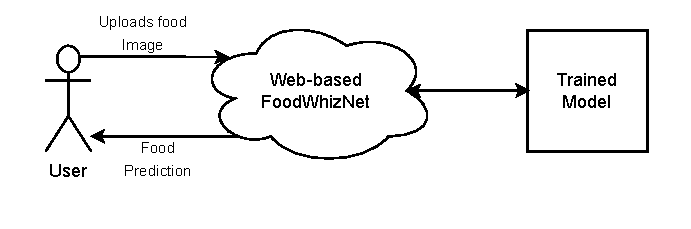
\includegraphics[width=1\textwidth]{graphics/images/deployment.pdf}
	\caption{Deployment}
	\label{fig:deploy}
\end{figure}
Shown in figure \ref{fig:deploy} is the usage of the web-based FoodWhizNet. A user is expected to upload a food image to the web application. Then, using the trained model in the backend, the image is classified accordingly and is returned to the client side of the web application and presented to the user. The best model of the study will be deployed through a web application with the front end to include CSS, HTML, and JavaScript. The backend will include the use of Flask to handle the model. A GitHub Pages will be utilized to host the web application.